% Layout for an independently distributed technical report.
\documentclass[manuscript,screen,nonacm]{acmart}
\setcopyright{none}
\settopmatter{printacmref=false,printccs=false}
\acmDOI{}
\acmISBN{}
\usepackage{longtable,booktabs,array,calc}
\usepackage{xurl}
\usepackage{fvextra}
\DefineVerbatimEnvironment{verbatim}{Verbatim}{breaklines=true,fontsize=\small}
\usepackage{tikz}
\usetikzlibrary{positioning}
\providecommand{\tightlist}{\setlength{\itemsep}{0pt}\setlength{\parskip}{0pt}}
\providecommand{\passthrough}[1]{#1}
\providecommand{\pandocbounded}[1]{#1}
\usepackage{graphicx,float}

% Permit figures to share pages with surrounding explanatory text.
\renewcommand{\topfraction}{0.92}
\renewcommand{\bottomfraction}{0.85}
\renewcommand{\textfraction}{0.06}
\renewcommand{\floatpagefraction}{0.80}
\setcounter{topnumber}{3}
\setcounter{bottomnumber}{3}
\setcounter{totalnumber}{5}
\setlength{\textfloatsep}{12pt plus 2pt minus 3pt}
\setlength{\intextsep}{12pt plus 2pt minus 3pt}
\raggedbottom

\geometry{top=0.75in,bottom=0.65in,includeheadfoot}
\begin{document}
\title{AFFECTOR: Coordinate-Guided Text Rewriting through Transformer
Activation Interventions}
\author{William Taggart}
\affiliation{\department{Modern and Classical Languages and Literatures}
\institution{Virginia Tech}\city{Blacksburg}\state{Virginia}\country{USA}}
\email{wtaggart@vt.edu}
\subtitle{Technical Report: November 14, 2026}
\begin{abstract}
AFFECTOR investigates whether a prescribed emotional trajectory can
influence the rewriting of a document. A trajectory assigns valence,
emotional direction, and intensity to normalized positions in a text. A
local backend maps these coordinates into perturbations of a frozen
language model's internal states, while hosted backends use
coordinate-bearing instructions. The desktop application supports
geometry authoring, editable numerical steering matrices, document
conversion, checkpointing, and separate emotional verification. This
paper derives the implemented method from first principles and
distinguishes mechanical correctness from successful emotional transfer.
Current controls can produce emotionally charged language but can also
produce weak paraphrases, factual distortions, and repetition. The
implementation is an experimental instrument, not a validated predictor
or controller of human emotion.
\end{abstract}
\keywords{activation steering, emotional text generation, transformer models, controllable generation}
\maketitle
\section{Purpose and Research Context}\label{literature-review-activation-steering-and-emotion}\label{problem-formulation}

A document conveys more than propositions. Its lexical choices, rhythm, imagery, focus, and narrative stance also shape how a reader feels as the text unfolds. AFFECTOR begins with a practical question about that progression: can a writer specify a desired emotional path and use it to guide a rewrite, while choosing how much of the original content to preserve? To make this question tractable, the application represents the path as an ordered curve of valence, inward/outward emotional direction, and intensity across the document. This representation supplies a coarse target for experimentation, leaving the model to realize it in language. The resulting text must therefore be judged both by its emotional fit and by its readability, content changes, and length.

Activation steering offers a way to connect this target to the process of generation. Turner and colleagues construct intervention vectors from contrasting prompts, while Panickssery and colleagues average activation differences across positive and negative behavioral examples \cite{turner2023actadd,panickssery2024caa}. Building on this contrastive approach, AFFECTOR maps emotional coordinates into changes to a frozen model's internal states during local inference. The application also provides an API route, in which the coordinates are expressed as instructions to a hosted model. Together, these routes make it possible to investigate numerical intervention alongside prompt-based control, although their settings and outcomes are not directly interchangeable.

\begin{figure}[!htb]
\centering
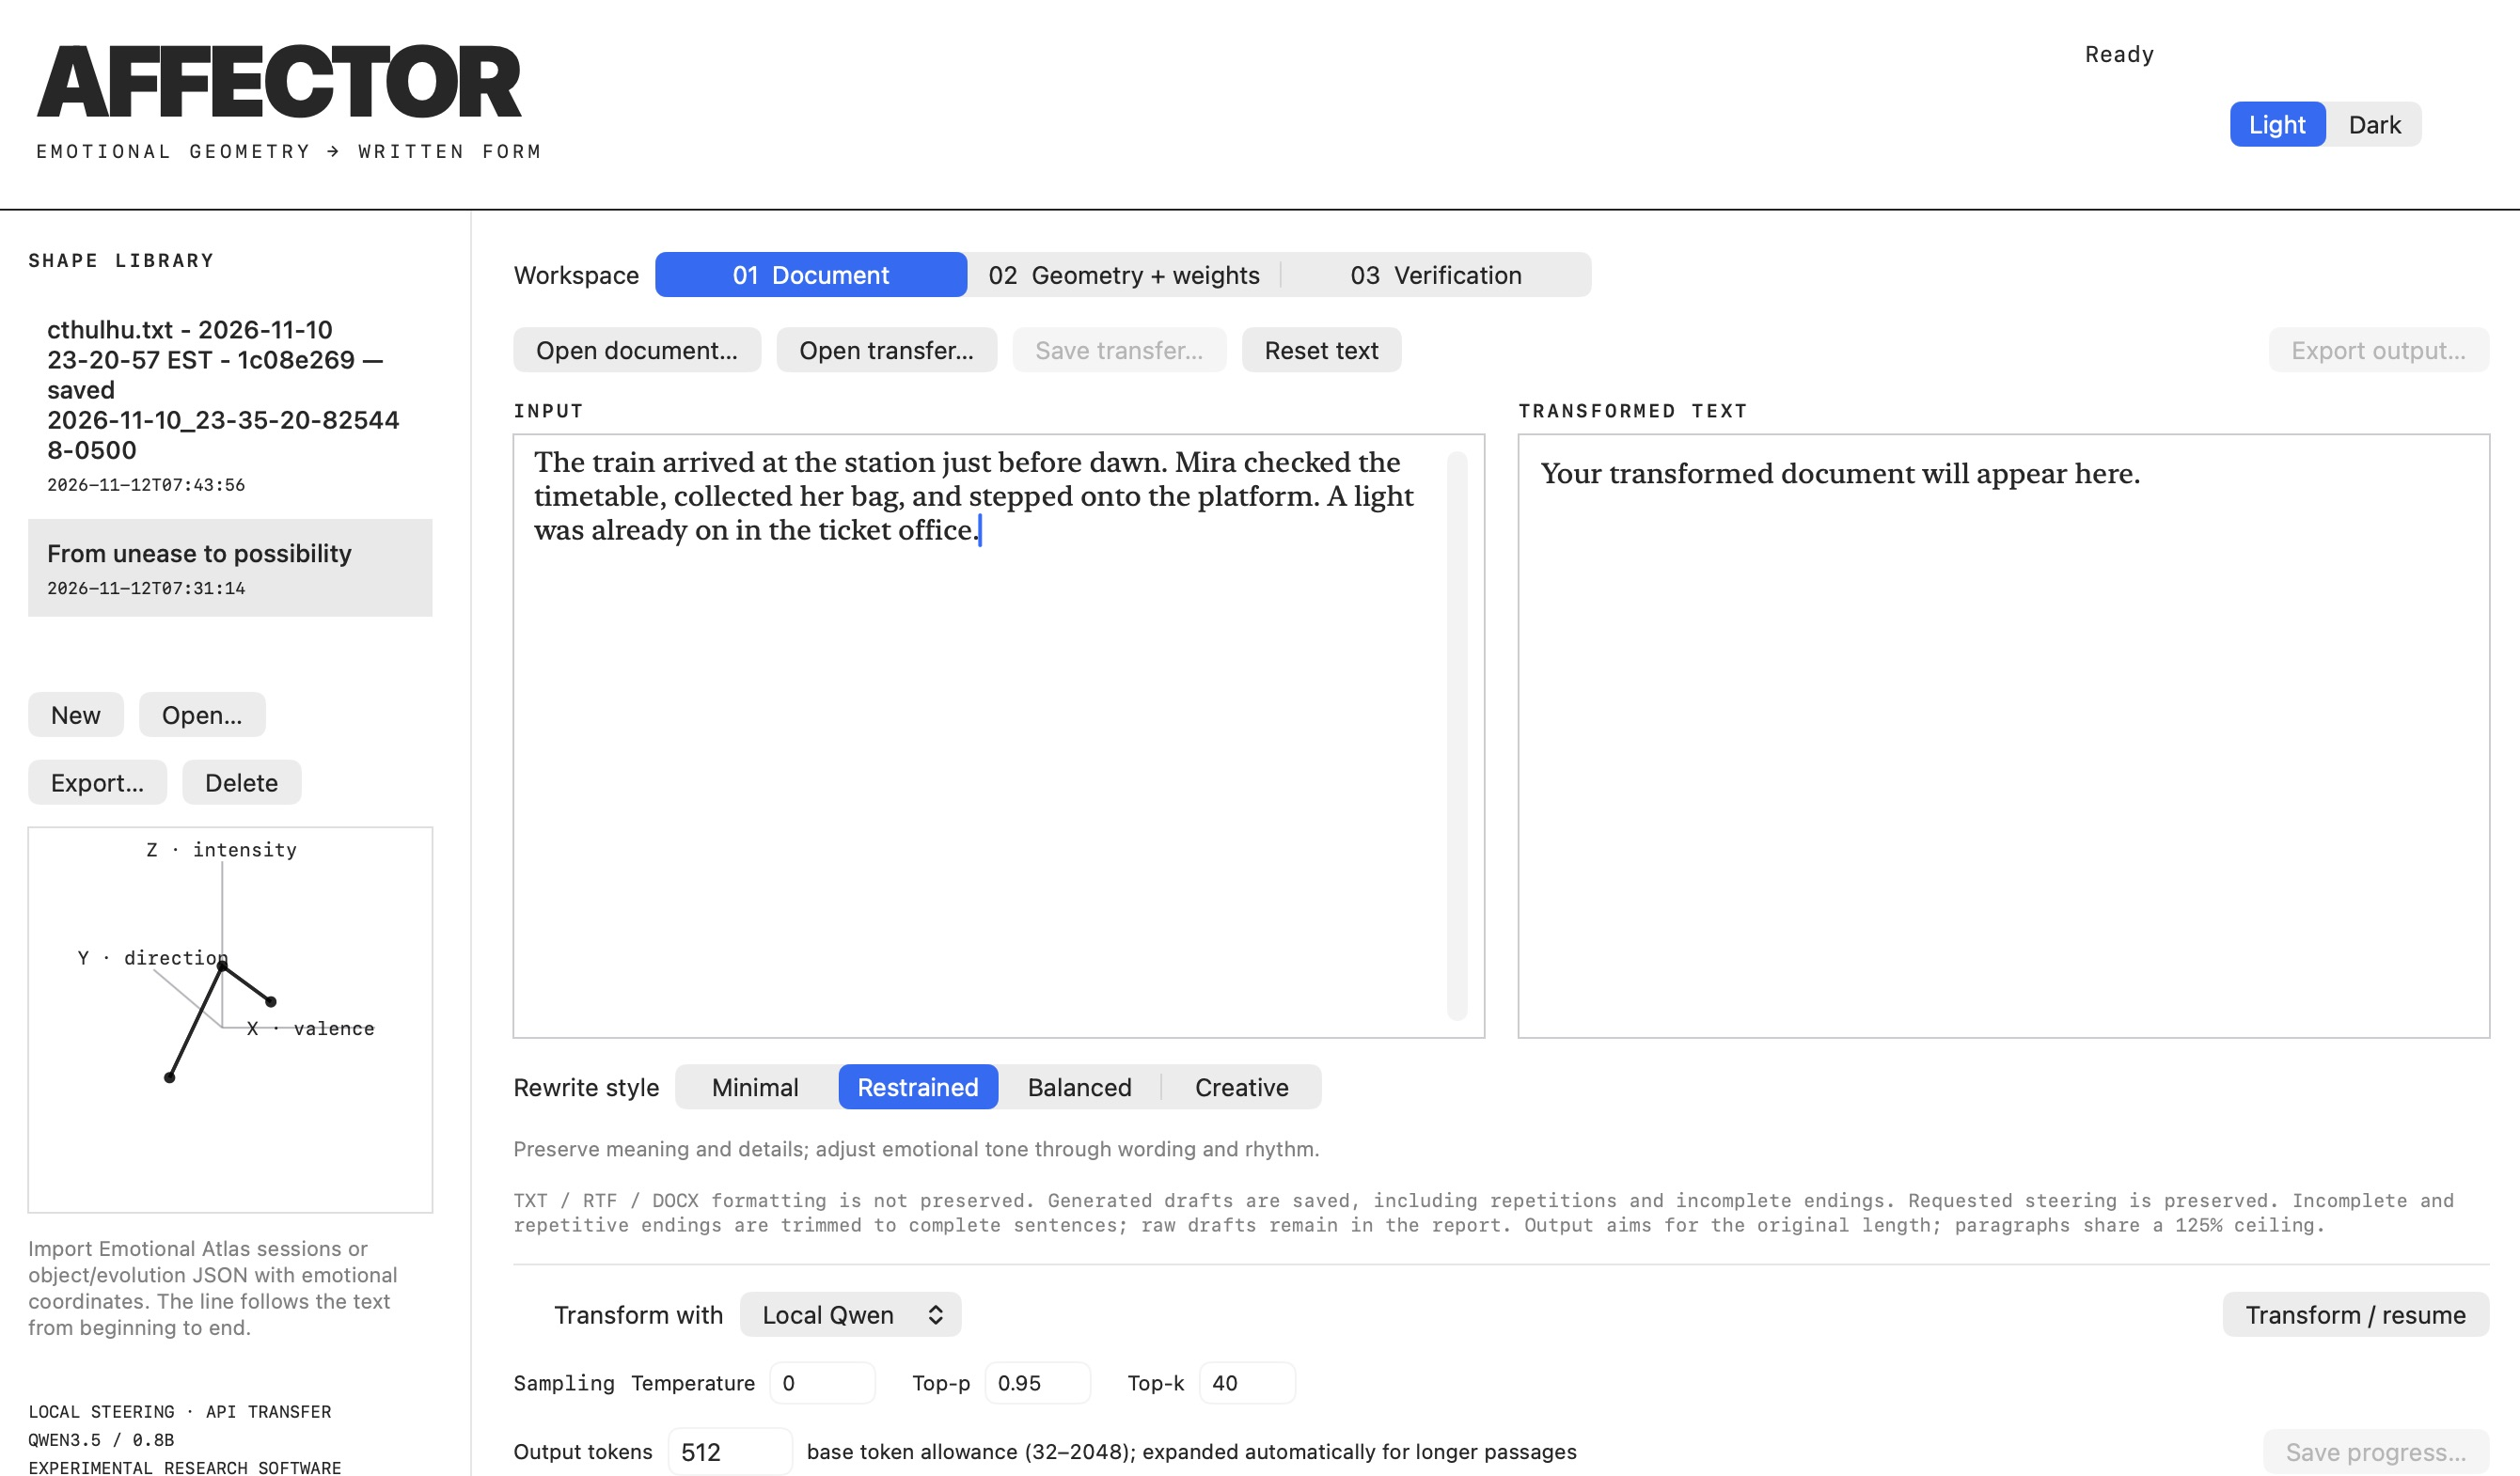
\includegraphics[width=.86\linewidth,height=0.58\textheight,keepaspectratio]{figures/screenshot-01.png}
\caption{Document workspace with an example input, rewrite controls, and an empty output pane before generation.}
\Description{Document workspace with an example input, rewrite controls, and an empty output pane before generation.}
\label{fig:app-screen-1}
\end{figure}

For either route, the usefulness of the coordinates depends on their relationship to human interpretations of the output. Work by Wu and colleagues connects model emotion spaces with human valence/arousal ratings and reports concept-based steering across linguistic-cultural settings \cite{wu2025emotion}. Diallo and colleagues extend this evaluative perspective by examining emotional intensity and text quality with human raters, finding effects that vary with the emotion and steering strength \cite{diallo2026style}. These findings motivate assessing emotional movement and readable expression separately. They also clarify what remains to be established for AFFECTOR: neither its inward/outward axis nor the correspondence between its RMS-scaled controls and a reader's emotional judgment has been validated by those studies.

This uncertainty concerns the intervention itself as well as its evaluation. Shu and colleagues find uneven causal organization across emotion categories in a study of sparse features and emotion recognition, while Wang and colleagues show that strong emotion-probing accuracy need not identify the best intervention layers in omni-modal models \cite{shu2026emotion,wang2026readbest}. Thus, recognizing an emotion in a representation does not by itself determine where to intervene to change it. The partially coupled supportive-empathy directions reported by Ha and colleagues further raise the question of whether changing one emotional dimension also moves another \cite{ha2026empathy}. Research on automated vector extraction and context-dependent strength offers ways to investigate these problems, with benefits that depend on the task and intended trade-off \cite{cui2025pas,ferrando2025dsas}. AFFECTOR exposes layer choices and coordinate mixtures as experimental controls; testing their interactions and potential adaptation remains part of the research agenda.

When these interventions are applied throughout a document, their effects must also be considered over the course of generation. E-STEER reports non-monotonic relationships between emotional interventions and outcomes in reasoning, generation, safety, and agent behavior \cite{sun2026emotion}. Similarly, Jeong's small-model comparison finds both coherent emotional changes and degeneration, including repetition, depending on the architecture and extraction method \cite{jeong2026emotion}. These results explain why greater intervention strength cannot simply be equated with a closer emotional match. In response to this practical difficulty, AFFECTOR combines bounded generation with records of repetition, truncation, and failed attempts. Its rewrite styles also let the user state how much content preservation should constrain the transformation, making that trade-off explicit when reviewing an output.

Taken together, these considerations define the scope of the present report: the implemented transformation pipeline, the choices it exposes, and the limits visible in its operation. Emotional verification is a separate user-invoked step; the application does not automatically score each passage and iteratively minimize its distance from the target. A broader assessment must therefore compare the requested progression with independently judged outcomes. SteerScope provides a useful framework by evaluating efficacy alongside side effects, generalization, and dependence on steering data \cite{yang2026steerscope}. Its finding that activation methods do not dominate prompt steering in the tested trade-offs supports including prompt-only and unsteered baselines, blinded emotional and quality ratings, and complete failure accounting. Such comparisons would establish whether AFFECTOR's controls offer a reliable advantage for particular writing tasks; they remain research requirements rather than completed evidence of effectiveness.

\section{Representation and
alignment}\label{representation-and-alignment}


\begin{figure}[!htb]
\centering
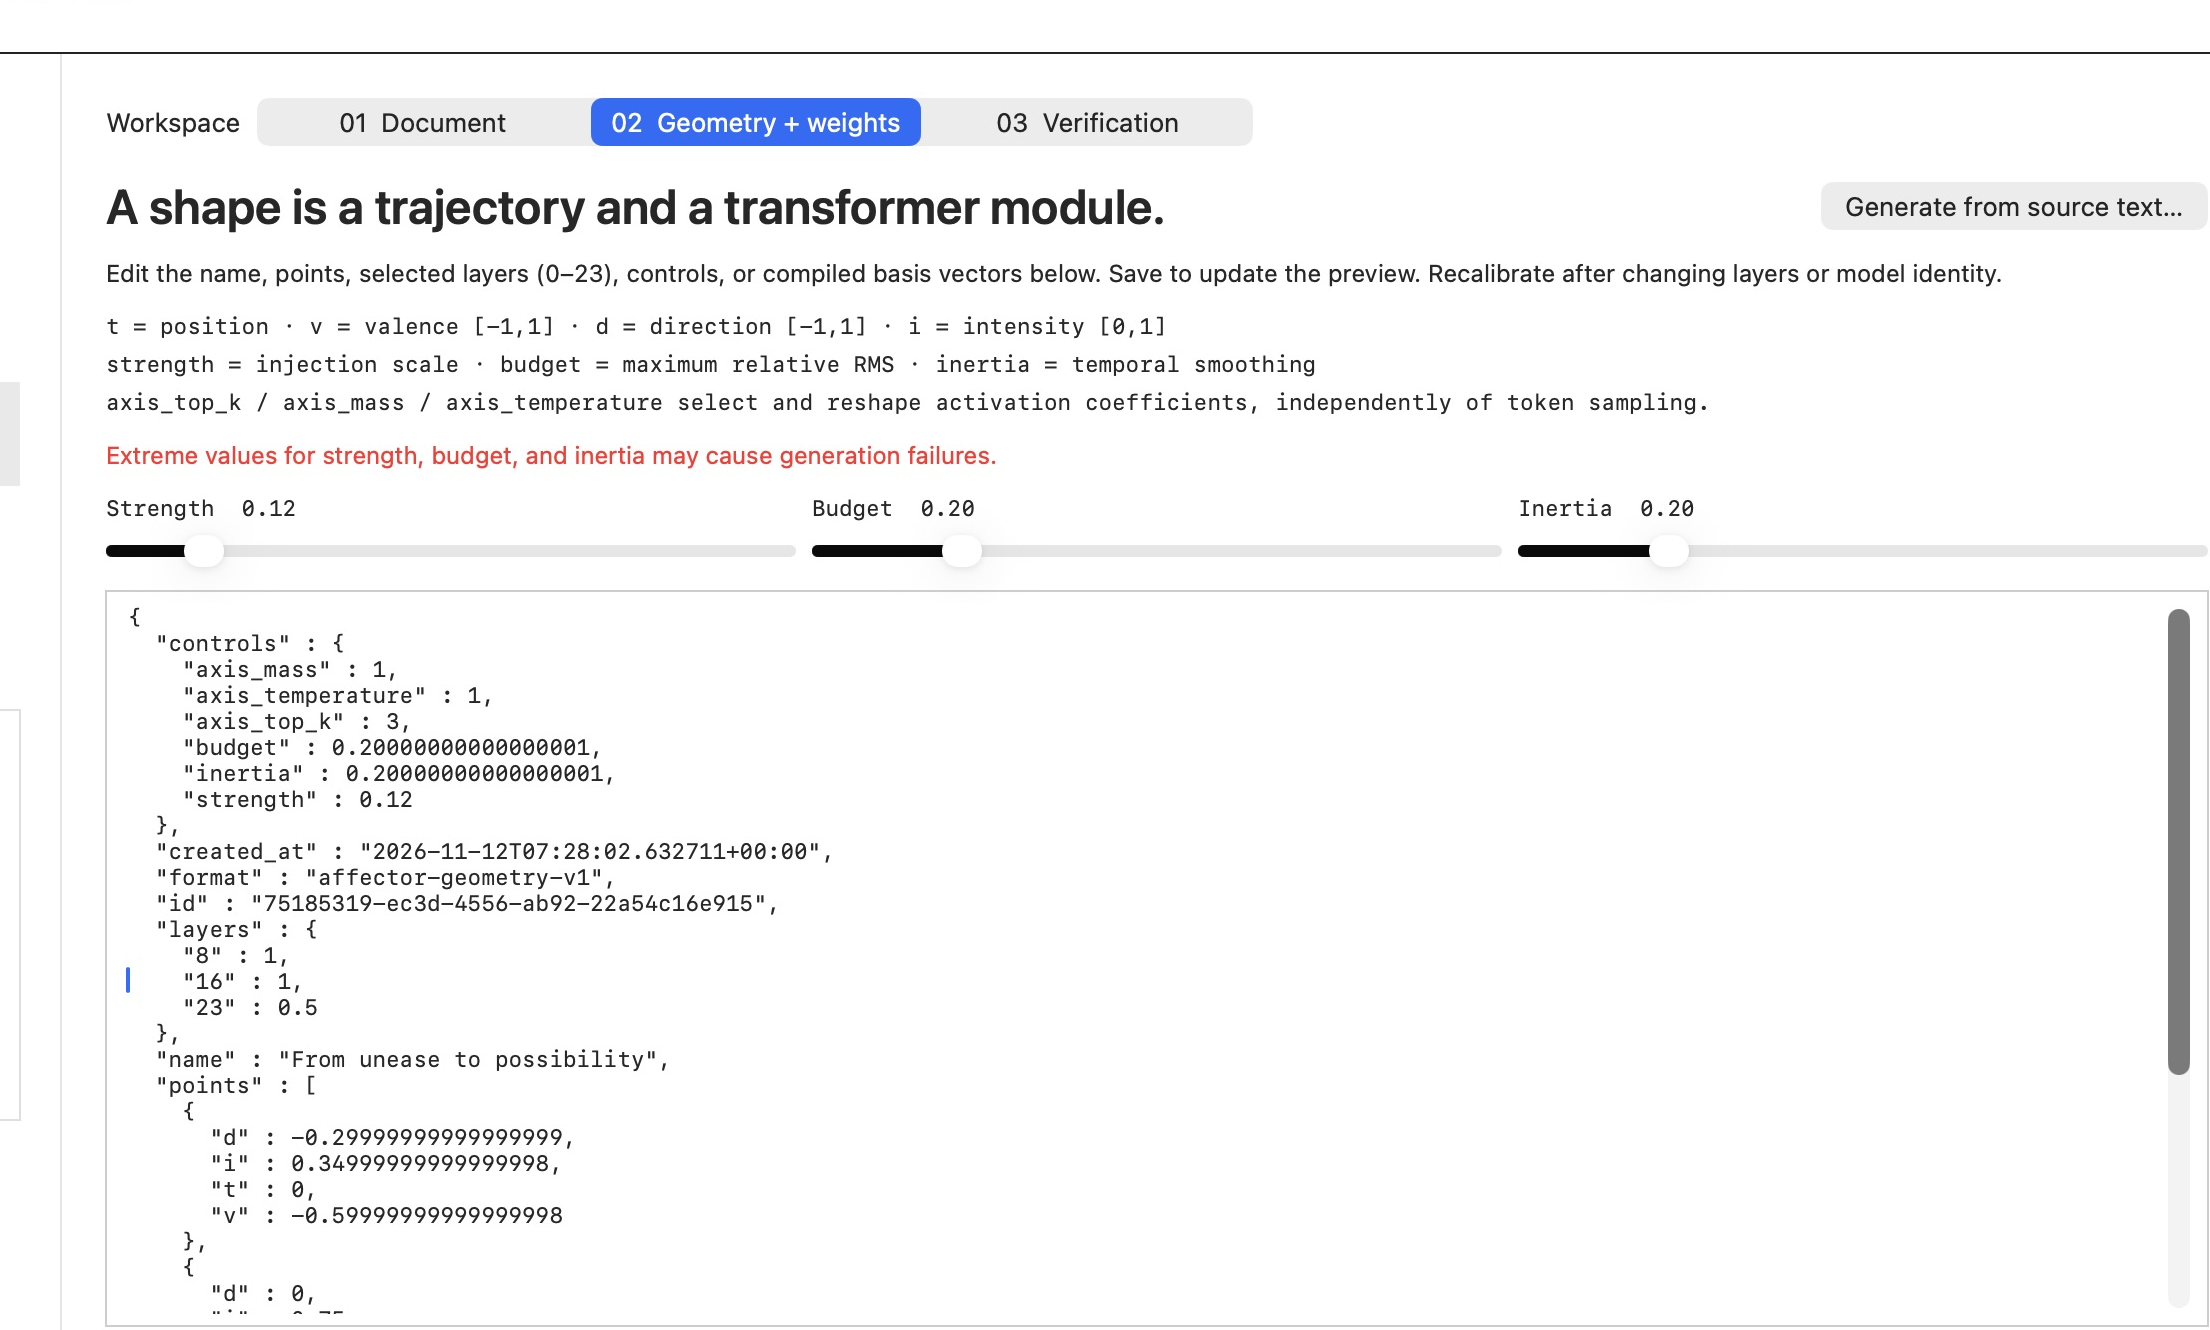
\includegraphics[width=.86\linewidth,height=0.58\textheight,keepaspectratio]{figures/screenshot-02.png}
\caption{Geometry editor showing the selected three-point trajectory and its steering controls.}
\Description{Geometry editor showing the selected three-point trajectory and its steering controls.}
\label{fig:app-screen-2}
\end{figure}
A geometry consists of ordered points \nolinkurl{(t, v, d, i)}. Position
\nolinkurl{t} is in \texttt{{[}0,1{]}}; valence \nolinkurl{v} and direction
\nolinkurl{d} are in \texttt{{[}-1,1{]}}; intensity \nolinkurl{i} is in
\texttt{{[}0,1{]}}. Negative valence denotes unpleasant affect and
positive valence pleasant affect. Negative direction denotes
self-focused or inward-directed emotion; positive direction denotes
outward focus. Direction is independent of valence: anger toward oneself
can be inward and sadness for another person outward. Intensity
describes strength of affect, not pleasantness.

For intervention, intensity is centered:

\[c(t)=(v(t),d(t),2i(t)-1).\]

Coordinates are linearly interpolated between points, with endpoint
clamping outside the stored range. Geometry imports that lack a
supported direction omit that point; interpolating across the resulting
gap can smooth away meaningful transitions. The imported data's
provenance records incomplete coverage.

The target document is divided into chunks of at most 700 characters,
preferring sentence endings and then whitespace. Blank-line paragraph
boundaries, including whitespace-only blank lines, are recognized. If a
chunk spans original character offsets \nolinkurl{a} through \nolinkurl{b} in
an input of length \nolinkurl{N}, its target position is
\nolinkurl{(a+b)/(2N)}. This is computed from the original document, so
expansion of earlier output does not move later targets. A single
coordinate is applied throughout a chunk. Neighboring chunks are
generated independently without surrounding text as generation context.

This normalized alignment compresses or stretches a source trajectory to
the target length. It samples only as many positions as there are
chunks. It does not preserve all events or oscillations of a much longer
curve. Changes to segmentation can change emotional targets even when
the same geometry is selected.

\begin{figure}[!htb]
\centering
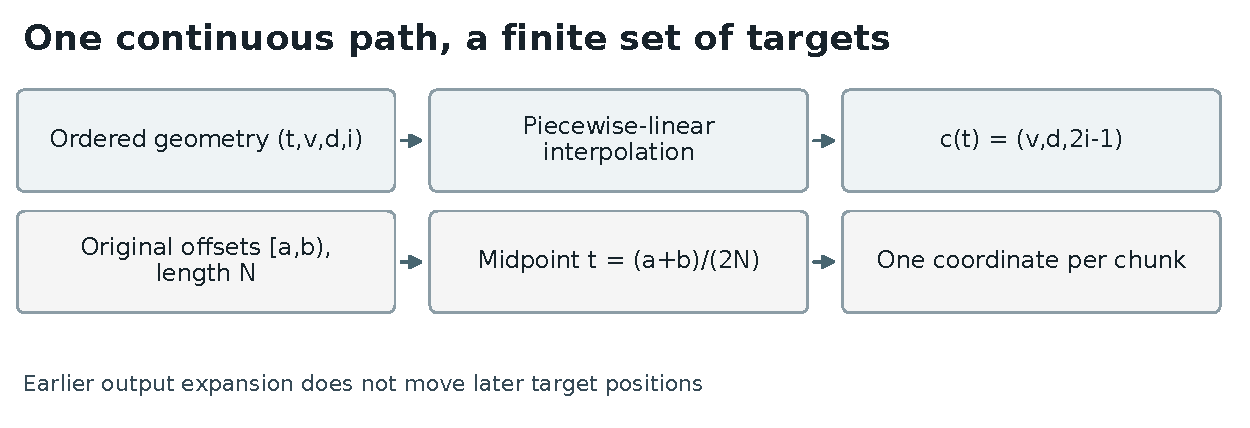
\includegraphics[width=.9\textwidth]{figures/illustration-01.pdf}
\caption{Normalized alignment schematic. Target chunks sample a continuous source path at original character midpoints; a short target can miss narrow changes in a long source trajectory.}
\Description{One continuous path, a finite set of targets. Normalized alignment schematic. Target chunks sample a continuous source path at original character midpoints; a short target can miss narrow changes in a long source trajectory.}
\label{fig:illustration-1}
\end{figure}

\section{Frozen model and contrastive
calibration}\label{frozen-model-and-contrastive-calibration}


\begin{figure}[!htb]
\centering
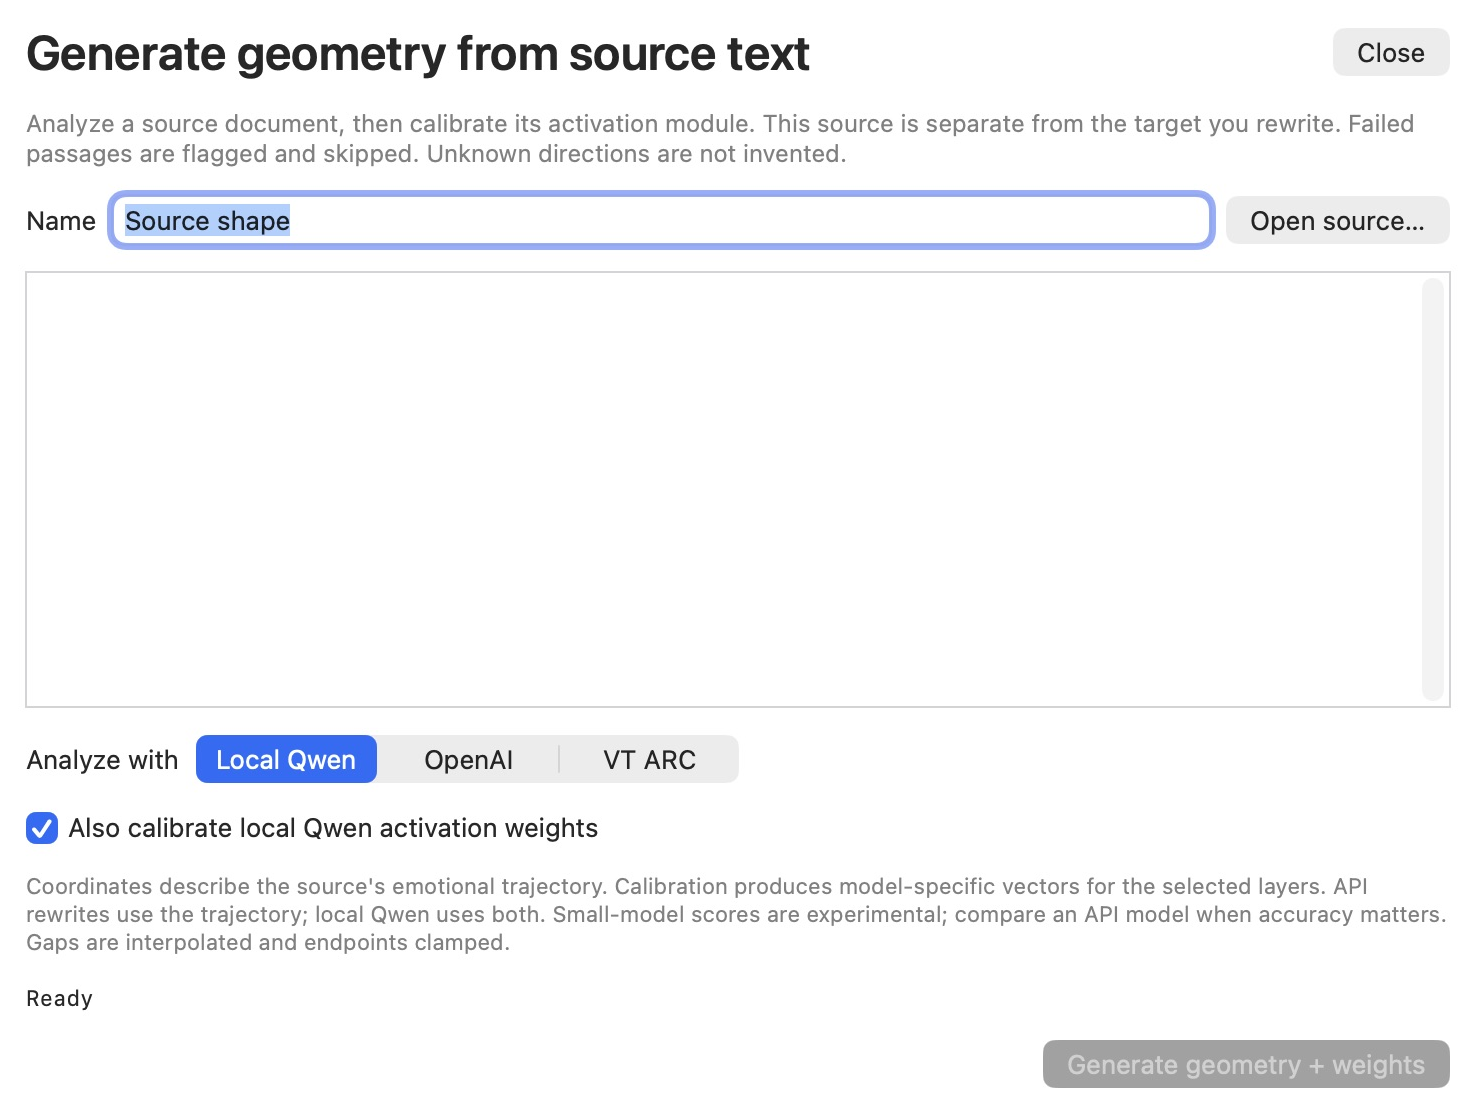
\includegraphics[width=.86\linewidth,height=0.58\textheight,keepaspectratio]{figures/screenshot-03.png}
\caption{Source-analysis dialog for generating a geometry and optionally calibrating a local activation basis.}
\Description{Source-analysis dialog for generating a geometry and optionally calibrating a local activation basis.}
\label{fig:app-screen-3}
\end{figure}
The local backend loads Qwen3.5-0.8B at revision
\nolinkurl{2fc06364715b967f1860aea9cf38778875588b17}. The implementation
operates on its text stack of 24 blocks with hidden width 1,024. Base
parameters are frozen; inference uses float32 and eager attention. Apple
MPS is selected when available, otherwise CPU. The chat template
disables thinking output. The package contains Python 3.14, PyTorch
2.15.0 and Transformers 5.22.2; exact dependency pins accompany the
bundle.

Before steering, the application obtains three directions per selected
layer from twelve manually authored English contrast pairs, four per
axis. For example, valence pairs contrast despair with joy, and
intensity pairs contrast mild unease with overwhelming terror. Both
members of every pair are processed under a continuation instruction.
Thus calibration requires 24 forward passes.

The capture site is the final chat-formatted prompt position immediately
before the post-attention normalization that feeds the feed-forward
sublayer. It is not a mean over all content tokens. For layer \nolinkurl{l}
and axis \nolinkurl{j}, the mean contrast is:

\[u_{\ell,j}=\frac14\sum_k(h^+_{\ell,j,k}-h^-_{\ell,j,k}).\]

With \texttt{RMS(x)\ =\ sqrt(mean\_r(x{[}r{]}\^{}2))}, normalization
gives:

\[B_{\ell,j}=\frac{u_{\ell,j}}{\max(\operatorname{RMS}(u_{\ell,j}),10^{-8})}.\]

The resulting \texttt{B{[}l{]}} is a 3 by 1,024 matrix. These are the
editable steering-module weights. Defaults select layers 8, 16, and 23,
with weights 1, 1, and 0.5. Geometry files retain the calibration
examples, matrices, and model/runtime identity; incompatible identities
are rejected.

There is no gradient training, score-supervised fitting,
orthogonalization, or guarantee that the three directions isolate their
intended concepts. Small hand-authored pairs can confound affect with
genre, topic, lexical content, and emotional categories. Calibration is
exploratory and English-based; multilingual effectiveness has not been
established.


\section{Coordinate-to-activation
computation}\label{coordinate-to-activation-computation}


\begin{figure}[!htb]
\centering
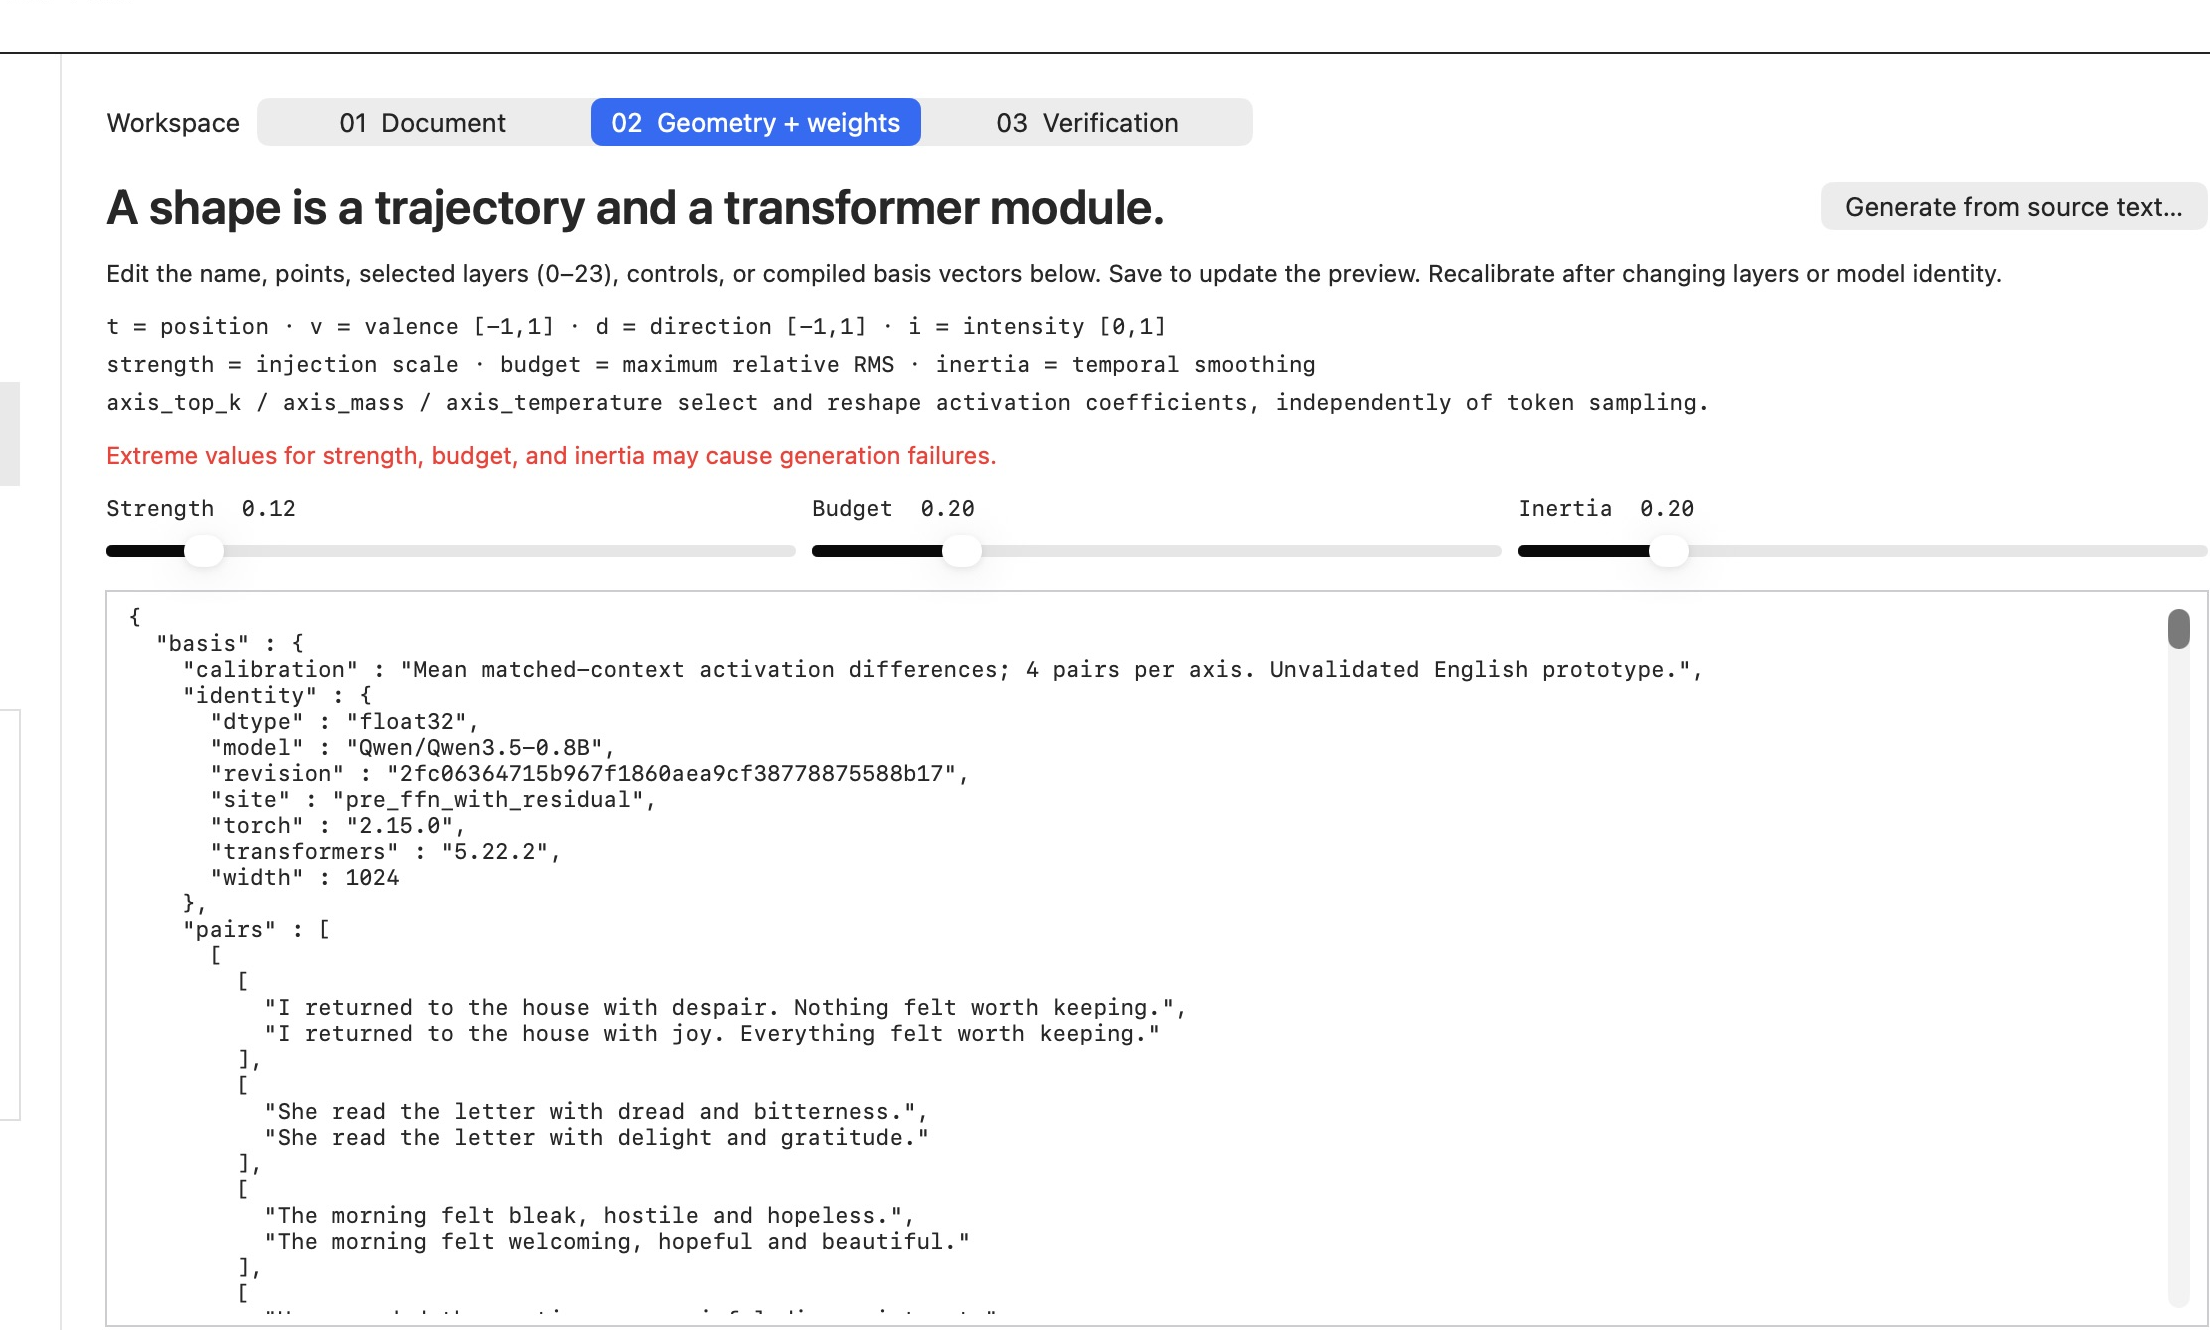
\includegraphics[width=.86\linewidth,height=0.58\textheight,keepaspectratio]{figures/screenshot-04.png}
\caption{Expanded numerical weights for the selected geometry, including the local calibration metadata.}
\Description{Expanded numerical weights for the selected geometry, including the local calibration metadata.}
\label{fig:app-screen-4}
\end{figure}
Axis temperature \nolinkurl{T} transforms each coordinate magnitude while
retaining its sign:

\[q_j=\operatorname{sign}(c_j)|c_j|^{1/T}.\]

The implementation ranks axes by magnitude, retains at most axis top-k,
and stops adding axes once cumulative magnitude reaches the configured
mass fraction. Surviving coefficients are not renormalized. These
operations act on three emotional coefficients, not on the model's
vocabulary distribution.

For current final-token hidden state \nolinkurl{h}, strength \nolinkurl{s},
and layer weight \texttt{w{[}l{]}}, the proposed perturbation is:

\[\delta_{\mathrm{raw}}=(q B_\ell)\operatorname{RMS}(h)s w_\ell.\]

Inertia \nolinkurl{rho} combines this proposal with the previous applied
perturbation within the same chunk:

\[\delta_{\mathrm{mix}}=\rho\delta_{\mathrm{previous}}+(1-\rho)\delta_{\mathrm{raw}}.\]

The first step uses the raw proposal directly. A relative RMS budget
\nolinkurl{beta} then bounds the perturbation:

\[\delta=\delta_{\mathrm{mix}}\min\left(1,\frac{\beta\operatorname{RMS}(h)}{\max(\operatorname{RMS}(\delta_{\mathrm{mix}}),10^{-12})}\right).\]

Zero strength, budget, or layer weight gives an exact zero perturbation.
Each chunk resets inertia history. The settings are applied as
requested; the release does not automatically lower them after poor
output.

Budget is not a semantic-change percentage. At budget 1, the
perturbation can have RMS magnitude comparable to the original hidden
state at that site. Large values can destabilize generation. Raising the
budget only matters when the proposed perturbation would otherwise be
clipped; it cannot correct an inaccurate direction.


\section{Intervention within the
transformer}\label{intervention-within-the-transformer}

Let \nolinkurl{h} denote a block's residual state after its attention or
sequence-mixing stage. A conventional feed-forward residual update has
the form:

\[y=h+\operatorname{FFN}(\operatorname{Norm}(h)).\]

AFFECTOR implements:

\[y=(h+\delta)+\operatorname{FFN}(\operatorname{Norm}(h+\delta)).\]

A pre-hook on the feed-forward normalization adds \nolinkurl{delta} to its
input, and a post-hook on the block output adds the same \nolinkurl{delta}
to the residual branch. This is a forward-pass intervention, not a
model-parameter update. Hooks affect only the final token in the initial
prompt pass and the current token during cached decoding. They are
removed when generation exits, including exceptional exits.

The module does not search for trigger phrases or recognize an idiom
before activating. The chosen target determines the intervention
continuously during decoding. Nevertheless, generation remains
conditional on the input and instruction, and the hidden state
influences perturbation magnitude. The module is not a
content-independent guarantee of a particular affect.

A key limitation is that the intervention is an absolute-coordinate
bias, not a measured error correction. A target valence of zero yields
no direct valence-axis perturbation; it does not actively neutralize an
already negative passage. Correlations between basis vectors further
complicate interpretation.


\section{Prompts, sampling, and bounded
output}\label{prompts-sampling-and-bounded-output}

Four rewrite styles constrain the instruction: Minimal preserves nearly
all wording; Restrained asks for subtle emotional phrasing changes while
preserving facts and structure; Balanced allows structural changes and
modest imagery while preserving events; Creative permits changes to
meaning, imagery, and events. The prompt preferences do not enforce
semantic fidelity.

Local prompts do not include the numerical emotional coordinates. Hosted
prompts do, because hosted model hidden states are not accessible
through the implemented APIs. Consequently, local and API modes are not
controlled comparisons of model size alone.

Temperature, top-p, and top-k govern token selection. At temperature
zero, decoding is greedy and top-p/top-k are inactive. Positive
temperature enables sampling. A repetition penalty of 1.1 and no-repeat
8-gram constraint operate on token decoding; they are distinct from
activation steering and cannot guarantee freedom from repetition.

The current output policy uses a shared paragraph allowance equal to
125\% of original character length. Unused allowance carries forward to
later chunks in the same paragraph; original intervening whitespace
counts against it. Earlier chunks cannot borrow from future chunks.
Local generation seeks a sentence ending after 85\% of the current
original chunk length. A hard character ceiling, token ceiling, and
120-second limit remain. Token allowances may expand above the displayed
base allowance, up to 2,048 locally and 4,096 for hosted requests.

Repetition detection inspects recent word n-grams and repeated character
patterns. If a draft is repetitive, oversized, or unfinished, the output
can retain only its complete, non-repetitive sentence prefix, with a
warning. If no such prefix exists, the original is retained with an
error. One generation attempt is made per chunk; returned drafts,
effective controls, stop reasons, and selection information remain in
reports. API calls are non-streaming, so their remote generation cannot
be stopped at an exact character threshold.

These mechanisms trade completeness for bounded readable output.
Sentence punctuation is a heuristic and can misidentify abbreviations or
unusual writing. Trimming can omit important content and alter emotional
character. They are safeguards against specific generation failures, not
a proof of success.

\section{Independent verification}\label{independent-verification}



Verification assesses original and revised chunks separately with an
unsteered evaluator or an API model. The evaluator is instructed to
distinguish felt or conveyed emotion from mere emotion-word occurrence,
identify experiencers and emotional targets, and supply exact quoted
evidence. It returns valence, direction, intensity, emotional labels,
uncertainty, and concise explanations. Scores are interpretive
estimates, not psychometric measurements.

For assessed coordinate \nolinkurl{p=(v,d,2i-1)} and target \nolinkurl{c}, the
reported similarity is:

\[\operatorname{similarity}=1-\frac{\lVert p-c\rVert_2}{2\sqrt3}.\]

The denominator is the maximum distance across the three-dimensional
\texttt{{[}-1,1{]}} cube. Similarity is not a probability. Axis errors
are also reported. Unknown direction makes the three-axis distance
unavailable. Aggregate before/after comparisons use only paired valid
assessments and report coverage and failures. Missing assessments are
not assigned invented scores.

The same small model can assess its own output, but shared weaknesses
make independent evaluation preferable. A high similarity can coexist
with incoherence, factual errors, or undesirable content. The
implementation does not optimize this score during generation and does
not include a formal semantic-fidelity metric.


\section{Architecture, persistence, and
privacy}\label{architecture-persistence-and-privacy}

A native SwiftUI/AppKit interface communicates with a Python subprocess
through JSON lines; no listening local web server is needed. The desktop
app provides geometry management, document transformation, verification,
light/dark appearance, and numeric weight editing. TXT, RTF, and DOCX
handling preserves textual content rather than rich layout.

Atomic checkpoint writes store original input, offsets, geometry,
controls, output records, and verification. Run signatures include the
input, settings, geometry, style, and policy version so changed settings
do not silently resume incompatible work. Loading an older checkpoint
validates its stored spans instead of resegmenting it. Individual
generation or assessment failures are flagged without interrupting the
whole document. Explicit cancellation stops the run; an in-flight API
call can take until its timeout to return.

API keys are held in memory. Local mode processes text on the computer;
API mode sends relevant passages to the selected service. Checkpoints
contain potentially sensitive document text and should be treated
accordingly. The distributed package excludes personal checkpoints and
test documents.

\section{Evidence and limitations}\label{evidence-and-limitations}

The release's 26 automated tests cover behaviors including checkpoint
handling, style persistence, failure continuation, allowance accounting,
raw-draft retention, and preservation of requested controls. Earlier
development smoke checks established nonzero activation interventions,
zero-strength equivalence under greedy decoding, hook cleanup, and the
RMS budget bound. These checks establish implementation properties, not
emotional efficacy.

Exploratory development runs revealed three important failure modes:
high intervention magnitudes can produce repetition before any full
sentence; lower magnitudes can yield fluent but weakly emotional
paraphrases; and segmentation changes alter which positions of a
trajectory are sampled. A temporary whole-paragraph/reduced-steering
recovery design improved completion on a small example but weakened the
desired affect, and is not the current release behavior.

No representative benchmark, blinded human study, multilingual
evaluation, or statistically supported success rate is claimed.
Controlled experiments should hold input, geometry, prompt,
segmentation, and sampling constant while comparing unsteered and
steered output. Report emotional distance, completion rate, repetition,
length ratio, factual/content preservation, and human judgments
together. Selection based on emotional distance alone can reward extreme
or incoherent writing.

\section{Conclusion}\label{conclusion}

AFFECTOR makes a low-dimensional emotional trajectory operational
through explicit transformer-state interventions and a separate
prompt-based backend. Its value is as an inspectable experimental
system: coordinates, editable vectors, controls, raw drafts, and
verification are exposed. Reliable emotional transfer remains an
empirical research problem. The current method demonstrates a
controllable intervention mechanism but does not establish that a
particular intervention reliably creates a specified emotional
experience.

\section{Implementation and infrastructure
sources}\label{implementation-and-infrastructure-sources}

\begin{enumerate}
\def\labelenumi{\arabic{enumi}.}
\item
  Qwen team. Qwen3.5-0.8B model card and distribution.
  \url{https://huggingface.co/Qwen/Qwen3.5-0.8B}
\item
  PyTorch documentation. Module forward and forward-pre hooks.
  \url{https://docs.pytorch.org/docs/stable/generated/torch.nn.Module.html}
\item
  Hugging Face Transformers documentation. Text generation.
  \url{https://huggingface.co/docs/transformers/main_classes/text_generation}
\item
  Apple Developer documentation. Notarizing macOS software before
  distribution.
  \url{https://developer.apple.com/documentation/security/notarizing-macos-software-before-distribution}
\end{enumerate}

The equations and implementation descriptions above are derived from the
included source. Upstream documentation describes infrastructure and
model distribution, not evidence validating AFFECTOR's
emotional-transfer claims.

\section*{AI assistance disclosure}
This project was created with assistance from GPT-6 Astra and Codex. AI
tools supported software development, testing, and the drafting and
revision of this technical report. William Taggart is responsible for
the project's research decisions and the final software and
documentation. AI assistance does not constitute independent validation
of the implementation or its scientific claims; the validation evidence
and limitations are stated separately in this report.

\bibliographystyle{ACM-Reference-Format}
\bibliography{references}

\section*{Suggested citation}
William Taggart. 2026. AFFECTOR: Coordinate-Guided Text Rewriting
through Transformer Activation Interventions. Technical report. Modern
and Classical Languages and Literatures, Virginia Tech. November 14, 2026.
\url{https://huggingface.co/will-taggart/AFFECTOR/blob/main/docs/TECHNICAL_PAPER.md}

\end{document}
